\section{Introduction} % A complete overview

% DONE Introduces the larger reasearch area that the paper is part of
% DONE Illustrates the concrete problem
% Explains the proposed solution
% Highlights the main results
% Might finish with a short explanation of the following sections

In computer architecture, the ``memory wall''~\cite{wulf_mckee_1995}
is a well known problem. Slow memory act as a bottleneck in a system
with fast processors. The reason for this is that processors will
request data faster than what primary memory can provide. In a Von
Neumann architecture~\cite{von1992first}, the processor
will stall as it waits for the next data or instruction to arrive.

\begin{center}
  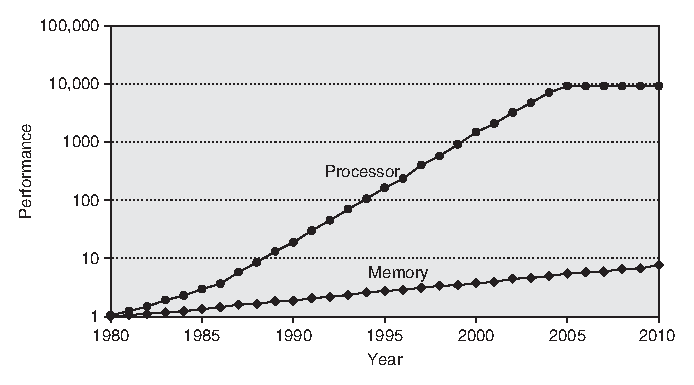
\includegraphics[width=0.5\textwidth]{graphs/memorywall}
  \captionof{figure}{The Memory Wall}
\end{center}

To better utilize the available processing power, CPU stalling for
memory operations needs to be avoided. Stalls occur because loading
data from main memory takes several cycles. We can avoid some of this
waiting by keeping often-used data in a special memory which is
smaller and faster than main memory, in addition to being closer to
the processor. This memory is called Cache memory.

Because we can't keep all main memory data in cache, we inevitably get
what is called cache misses. A cache miss happens when the requested
data is not found in cache, requiring the system to fetch the data
from main memory. This can waste hundreds of cycles. Therefore, the
number of cache misses should be minimized.

% There are several techniques used in modern systems which mitigates
% this bottleneck, like caching or outsourcing memory management to a
% DMA. One interesting approach is named ``prefetching''.

Prefetching involves speculating in which memory addresses are needed
in the near future, and fetching them into cache prior to
execution. This paper investigates the ``speculating'' part, that is,
what addresses should be fetched and when. When the prefetching is
successful, CPU stalling is avoided as the processor has the needed
data available, resulting in increased performance. When unsuccessful,
valuable cache space is wasted.

The most basic kind of prefetching would be to load the memory
addresses which sequentially follow the address we are currently
working on. However, this tends to be not so effective as memory
access tend to be non-sequential. Instead, we can look for access
patterns, and try to exploit them.

In this paper we start by exploring the sequential prefetcher. A
Stride Directed Prediction prefetcher, a slight improvement to the
previous is also implemented and tested. Later, two prefetchers which we have implemented are shown
and tested. The first is based on Chen and Baer's reference
prediction tables~\cite{chen_baer_1995} (with and without
lookahead). The third is based on Nesbit and Smith's Global History
Buffer with delta correlating~\cite{nesbit_smith_2005}. All
prefetchers have been benchmarked with SPEC CPU2000 in the M5
simulator.

% http://ieeexplore.ieee.org/abstract/document/5389383/
